% Shared standalone design for the editable figure reconstructions.
\documentclass[tikz,border=5pt,10pt]{standalone}
\usepackage[T1]{fontenc}
\usepackage[utf8]{inputenc}
\usepackage{newpxtext,newpxmath}
\usepackage[scaled=.94]{sourcesanspro}
\usepackage{pgfplots}
\pgfplotsset{compat=1.18}
\usetikzlibrary{arrows.meta,calc,positioning,decorations.pathreplacing,
  decorations.markings,patterns,matrix,shapes.geometric,fit,backgrounds,
  intersections,angles,quotes}
\definecolor{ink}{HTML}{203746}
\definecolor{accent}{HTML}{146C78}
\definecolor{muted}{HTML}{667780}
\definecolor{signalred}{HTML}{B94B44}
\color{ink}
\tikzset{>=Latex,line width=.8pt,
  every node/.style={font=\small},
  axis/.style={->,draw=muted,line width=.5pt},
  guide/.style={draw=muted,dashed,line width=.45pt},
  curve/.style={draw=accent,line width=1pt},
  marker/.style={circle,fill=accent,inner sep=1.5pt},
  labelbox/.style={fill=white,inner sep=2pt}}

\begin{document}
\begin{tikzpicture}[x=0.78cm,y=0.78cm,every node/.style={font=\footnotesize}]
\draw[accent!22,line width=.55pt] (0,0) ellipse (0.55 and 0.24596747752497689);
\draw[accent!22,line width=.55pt] (0,0) ellipse (1.1 and 0.49193495504995377);
\draw[accent!22,line width=.55pt] (0,0) ellipse (1.8 and 0.8049844718999243);
\draw[accent!22,line width=.55pt] (0,0) ellipse (2.6 and 1.1627553482998907);
\draw[accent!22,line width=.55pt] (0,0) ellipse (3.6 and 1.6099689437998486);
\draw[accent!22,line width=.55pt] (0,0) ellipse (4 and 1.7888543819998317);
\draw[accent,line width=1.1pt] (3.0000,1.1000)--(2.5500,0.2750)--(2.1675,0.0688)--(1.8424,0.0172)--(1.5660,0.0043)--(1.3311,0.0011)--(1.1314,0.0003)--(0.9617,0.0001)--(0.8175,0.0000)--(0.6949,0.0000)--(0.5906,0.0000);
\draw[signalred,dashed,line width=1.1pt] (3.0000,1.1000)--(1.8900,-0.9350)--(1.1907,0.7948)--(0.7501,-0.6755)--(0.4726,0.5742)--(0.2977,-0.4881)--(0.1876,0.4149)--(0.1182,-0.3526)--(0.0744,0.2997)--(0.0469,-0.2548)--(0.0295,0.2166);
\fill[accent] (3.0000,1.1000) circle (1.3pt);
\fill[accent] (2.5500,0.2750) circle (1.3pt);
\fill[accent] (2.1675,0.0688) circle (1.3pt);
\fill[accent] (1.8424,0.0172) circle (1.3pt);
\fill[accent] (1.5660,0.0043) circle (1.3pt);
\fill[accent] (1.3311,0.0011) circle (1.3pt);
\fill[accent] (1.1314,0.0003) circle (1.3pt);
\fill[accent] (0.9617,0.0001) circle (1.3pt);
\fill[signalred] (3.0000,1.1000) circle (1.3pt);
\fill[signalred] (1.8900,-0.9350) circle (1.3pt);
\fill[signalred] (1.1907,0.7948) circle (1.3pt);
\fill[signalred] (0.7501,-0.6755) circle (1.3pt);
\fill[signalred] (0.4726,0.5742) circle (1.3pt);
\fill[signalred] (0.2977,-0.4881) circle (1.3pt);
\fill[signalred] (0.1876,0.4149) circle (1.3pt);
\fill[signalred] (0.1182,-0.3526) circle (1.3pt);
\fill[ink] (3,1.1) circle (1.9pt) node[above right] {$x_0$};\fill[ink] (0,0) circle (1.8pt) node[below left] {$x^\star$};

\node at (0,2.65) {$f(x)=\tfrac12(x_1^2+5x_2^2)$};
\draw[accent,line width=1.1pt] (-3.7,-2.15)--(-3,-2.15);\node[anchor=west] at (-2.9,-2.15) {$\tau=0.15$};
\draw[signalred,dashed,line width=1.1pt] (.7,-2.15)--(1.4,-2.15);\node[anchor=west] at (1.5,-2.15) {$\tau=0.37$};
\node[align=center] at (0,-3) {A larger step can oscillate\\across the narrow direction};
\end{tikzpicture}
\end{document}
